\documentclass[8pt]{article}

%%%%%%%%%%%%%%%%
%%% Packages %%%
%%%%%%%%%%%%%%%%

\usepackage[utf8]{inputenc}
\usepackage[english]{babel}
\usepackage{graphicx}
\usepackage{epstopdf}
\usepackage{amsmath,amssymb,amsbsy,amsthm,color}
\usepackage[paperwidth=19cm,paperheight=29.7cm,hmargin=2cm,vmargin=3cm]{geometry}

\usepackage[square,numbers]{natbib}

% \graphicspath{{figures/}}


\begin{document}

\bibliographystyle{natbib}
	
\title{The Method of Lagrangian Descriptors}

\date{}
	
% \author{V. J. Garc\'{i}a-Garrido}
	
\maketitle

\vspace{-0.5cm}

One of the biggest challenges of Dynamical Systems Theory or Nonlinear Dynamics is the development of mathematical techniques that provide us with the capability of exploring the geometrical template of structures that governs transport in phase space. Since the early 1900, the idea of pursuing a qualitative description of the solutions of differential equations, which emerged from the pioneering work carried out by Henri Poincar\'e on the three body problem of Celestial Mechanics \cite{hp1890}, has had a profound impact on our understanding of the nonlinear character of natural phenomena. Indeed, this powerful approach has now been widely embraced by the scientific community and its essence was nicely captured by Vladimir Arnold's statement that a complete description of Classical Mechanics boils down to the geometrical analysis of phase space. 

In this chapter we present the details of a mathematical tool whose potential brings us  one step closer to fulfilling the long-soght dream envisioned by Poincar\'e. The method is known in the literature as Lagrangian descriptors (LDs) and has the capability of revealing the geometrical template of phase space structures that characterizes trajectories with qualitatively distinct dynamical behavior. As we will see, this method provides us with a systematic way of exploring phase space by means of looking at its dynamical skeleton using low-dimensional slices. This procedure allows for a complete reconstruction, i.e. a \textit{phase space tomography}, of the intricate geometry of underlying invariant manifolds that characterize transport mechanisms.

Consider a general time-dependent dynamical system given by the evolution law:
\begin{equation}
\dfrac{d\mathbf{x}}{dt} = \mathbf{v}(\mathbf{x},t) \;,\quad \mathbf{x} \in \mathbb{R}^{n} \;,\; t \in \mathbb{R} \;,
\label{gtp_dynSys}
\end{equation}
where the vector field satifies $\mathbf{v}(\mathbf{x},t) \in C^{r} (r \geq 1)$ in $\mathbf{x}$ and continuous in time. If the vector field does not depend on time, the system is called \textit{autonomous}, and it is \textit{non-autonomous} otherwise. For any initial condition $\mathbf{x}(t_0) = \mathbf{x}_0$ this system of differential equations has a unique solution with the same regularity as that of the vector field, which also depends continuously on the initial data \cite{coddington1984}. The vector field that defines the flow equations can be determined by an analytical model, or it could also have been retrieved from numerical simulations as a discrete spatio-temporal dataset. For instance, the vector field could represent the velocity field of oceanic or atmospheric current obtained from satellite measurements or from the numerical solution of Geophysical models. Intersestingly, and in the context of chemical reaction dynamics, the vector field could be the result of molecular dynamics simulations.

Our goal in this chapter is to give an introduction to the method of Lagrangian Descriptors, which has the capability of revealing the underlying template of geometrical structures that determine transport in phase space for the dynamical system in Eq. \eqref{gtp_dynSys}. The natural way to explore phase space structure is to use trajectoriess, since these objects are its building blocks. In fact, the geometry of phase space is enconded in the initial conditions themselves of all the trajectories of the system. The simple and elegant idea behind LDs in order to provide a qualitative description of the system's dynamics is to seed a given phase space region with initial conditions and integrate a bounded and positive quantity (an intrinsic geometrical and/or physical property of the dynamical system under study) along trajectories for a finite time. This approach for revealing the mathematical structures that make up the dynamical skeleton governing phase space transport, is remarkably similar to the visualization techniques developed in fluid mechanics experiments in the laboratory to uncover beautiful patterns of flow structures by studying the evolution of drops of dye injected into a moving fluid \cite{chien1986}. A powerful analogy can be found in the classical experiment where the magnetic field lines of a magnet become visible by employing iron filings that align with the magnetic field.

The method of Lagrangian Descriptors is a trajectory-based scalar diagnostic that was first introduced a decade ago to analyze Lagrangian transport and mixing in Geophysical flows \cite{madrid2009,mendoza2010}. In its origins, it was used as a tool to detect \textit{distinguished hyperbolic trajectories}, which are ``moving saddles'', a generalization of the concept of saddle fixed points of autonomous dynamical systems to the nonautonomous setting. As we will see shortly, the first definition of LDs relied on the computation of the arclength of the trajectories of initial conditions as they evolve forward and backward in time \cite{mendoza2010,mancho2013lagrangian}. Since its proposal as a nonlinear dynamics tool to explore phase space, this methodology has found a myriad of applications in different scientific areas. For instance, in the context of Geophysics, it has been used in Oceanography to plan transoceanic autonomous underwater vehicle missions by taking advantage of the underlying dynamical structure of ocean currents \cite{ramos2018}. Also, it has been shown to provide relevant information for the effective management of marine oil spills \cite{gg2016}. In the Atmospheric Sciences, this methodology has been used to analyze the structure of the Stratospheric Polar Vortex and its relation to sudden stratospheric warmings and also to ozone hole formation \cite{alvaro1,alvaro2,curbelo2019a,curbelo2019b}. In all these problems, the vector field defining the dynamical system is a discrete spatio-temporal dataset obtained from the numerical simulation of Geophysical models. Recently, this tool has also received recognition in the field of Chemistry, in particular in Transition State Theory \cite{craven2015lagrangian,craven2016deconstructing,craven2017lagrangian,revuelta2019unveiling}, where the computation of chemical reaction rates relies on the knowledge of the phase space structures that separate reactants from products. These high-dimensional structures characterizing reaction dynamics are typically related to Normally Hyperbolic Invariant Manifolds (NHIMs) and their stable and unstable manifolds that occur in Hamiltonian systems.

The method of Lagrangian descriptors, also known in the literature as function $M$, was originally defined in \cite{madrid2009} as the computation of the arclength of trajectories starting at the initial condition $\mathbf{x}(t_0)$ as they evolve forward and backward for a fixed intergation time $\tau$. The scalar function that defines this diagnostic has the form:
\begin{equation}
M(\mathbf{x}_{0},t_0,\tau) = \int^{t_0+\tau}_{t_0-\tau} ||\mathbf{v}(\mathbf{x}(t;\mathbf{x}_0),t)|| \; dt \;,
\label{M_function}
\end{equation}
where $||\cdot||$ is the Euclidean distance. Notice that the definition of function $M$  can be broken in a natural way into forward ($M^f$) and backward ($M^b$) integration:
\begin{equation}
M(\mathbf{x}_{0},t_0,\tau) = M^{b}(\mathbf{x}_{0},t_0,\tau) + M^{f}(\mathbf{x}_{0},t_0,\tau) \;,
\end{equation}
where we have that:
\begin{equation}
M^{f}(\mathbf{x}_{0},t_0,\tau) = \int^{t_0+\tau}_{t_0} ||\mathbf{v}(\mathbf{x}(t;\mathbf{x}_0),t)|| \; dt \;\;,\;\; 
M^{b}(\mathbf{x}_{0},t_0,\tau) = \int^{t_0}_{t_0-\tau} ||\mathbf{v}(\mathbf{x}(t;\mathbf{x}_0),t)|| \; dt \;.
\end{equation}
The advantage of splitting function $M$ into its forward ($M^f$) and backward ($M^b$) parts is that forward integration highlights the stable manifolds of the dynamical system, and backward evolution recovers the unstable manfifolds. Moreover, the combination of both forward and backward detects all the invariant manifolds simultaneously. The intuituitive idea why this tool works is that the influence of phase space structures on trajectories will result in differences (abrupt change) in arclength of nearby trajectories in the neighborhood of a phase space structure. The method nicely captures this distinct dynamical behavior allowing to recover the geometrical template of invariant manifolds that characterizes phase space transport. This detection of invariant manifolds by means of sharp changes in the scalar field values of LDs has been mathematically quantified in terms of the notion of ``singular structures'' in the LDs plots, which are easy to recognize visually \cite{mancho2013lagrangian,lopesino2017}. 

In order to apply LDs for revealing the invariant manifolds in phase space, it is very important to remark the crucial role played by the integration time $\tau$ in the definition of the method. The consequence of increasing the value for $\tau$ is that richer and more intricate details of the underlying geometrical template of phase space structures are unveiled. This behavior is expected, as an increase of the integration time would imply incorporating more information about the past and future dynamical history of trajectories in the computation of LDs. This means that $\tau$ is intimately related to the time scales of the dynamical phenomena that take place in the model under consideration and thus, it is a parameter that is problem-dependent. Hence, there is no general ``golden rule'' for selecting its value for exploring phase space, and consequently it is usually selected from the dynamical information obtained by performing beforehand several numerical experiments.

In the next example we illustrate how the arclength definition of LDs captures the stable and unstable manifolds that determine the phase portrait of the forced and undamped Duffing oscillator. The Duffing equation arises when studying the motion of a particle on a line, i.e. a one degree of freedom system, subjected to the influence of a symmetric double well potential and an external forcing. The second order ODE that describes this oscillator is given by:
\begin{equation}
\ddot{x} + x^3 - x = \varepsilon f(t) \quad \Leftrightarrow \quad 
\begin{cases}
\dot{x} = y \\
\dot{y} = x - x^3 + \varepsilon f(t) \\
\end{cases}
\end{equation}
where $\varepsilon$ measures the strength of the forcing term $f(t)$, and we choose for this example a sinusoidal force $f(t) = \sin(t)$. In the autonomous case, i.e. $\varepsilon = 0$, the system has three equilibrium points: a saddle located at the origin and two diametrally opoosed centers at the points $(\pm 1,0)$. The stable and unstable manifolds that emerge from the saddle point form two homoclininc orbits in the form of a figure eight around the two center equilibria:
\begin{equation}
\mathcal{W}^{s} = \mathcal{W}^{u} = \left\{(x,y) \in \mathbb{R}^2 \; \Big| \; 2y^2 + x^4 - 2x^2 = 0 \right\}
\label{duff_homocMani}
\end{equation}

We begin by computing LDs for the unforced Duffing system using $\tau = 2$. For this small integration time, the method highlights the saddle and center fixed points, since the arclength at those points is always zero. Moreover, in this case the phase portrait still looks blurry as shown in Fig. \ref{duffing1_lds} A), and this is a consequence of trajectories not having sufficient time to evolve in order to make distinct dynamical behaviors ditinguishable. If we now increase the integration time to $\tau = 10$, we can see in Fig. \ref{duffing1_lds} B) that the homoclinic connection formed by the stable and unstable manifolds of the saddle point at the origin becomes clearly visible. Moreover, observe that the manifolds are located at points where the scalar values taken by LDs change abruptly. This property is demonstrated in Fig. \ref{duffing1_lds} C), where we have depicted the value of function $M$ along the line $y = 0.5$. Notice that sharp changes in the scalar field of LDs at the manifolds are also related to local minima.

\begin{figure}[htbp]
	\begin{center}
		A)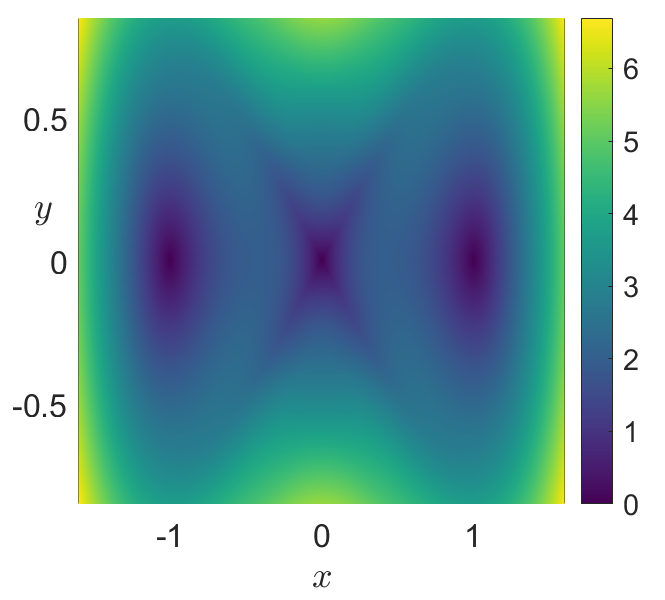
\includegraphics[scale=0.24]{duffing_tau_2.png}
		B)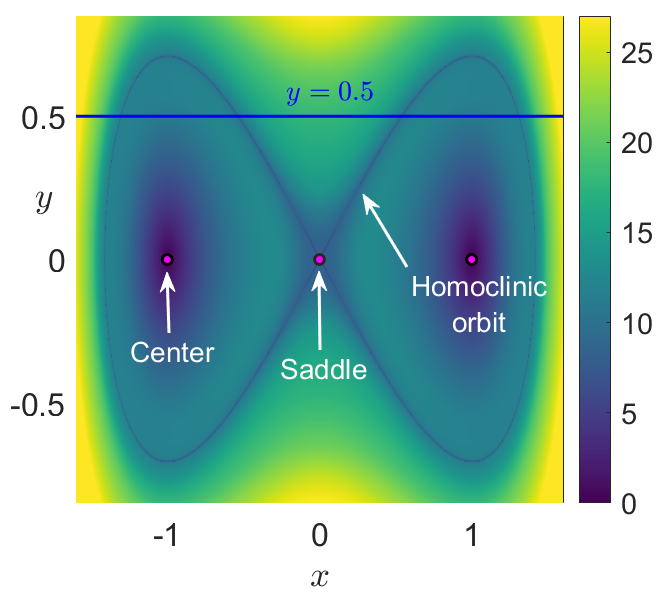
\includegraphics[scale=0.24]{duffing_tau_10.png}
		C)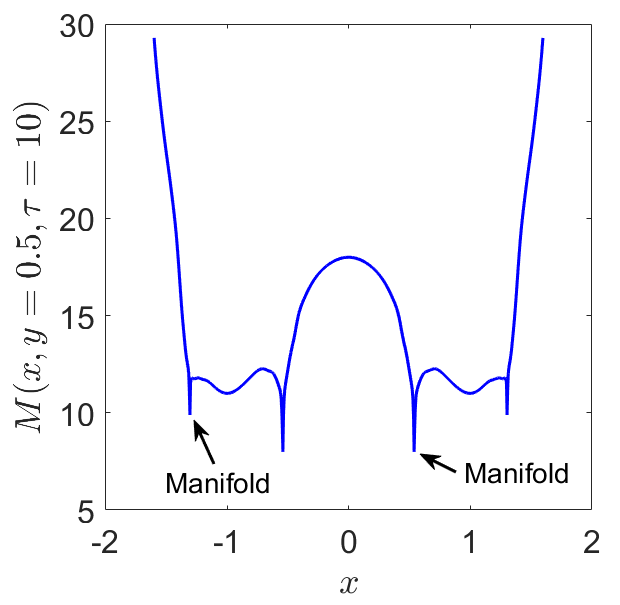
\includegraphics[scale=0.24]{duffing_maniDetect.png}
	\end{center}
	\caption{Phase portrait of the autonomous and undamped Duffing oscillator obtained by applying the arclength definition of LDs in Eq. \eqref{M_function}. A) LDs with $\tau = 2$; B) LDs with $\tau = 10$; C) Value of LDs along the line $y = 0.5$ depicted in panel B) illustrating how the method detects the stable and unstable manifolds at points where the scalar field changes abruptly.}
	\label{duffing1_lds}
\end{figure}

We move on to compute LDs for the forced Duffing oscillator. In this situation, the vector field is time-dependent and thus the dynamical system is nonautonomous. The consequence is that the homoclinic connection breaks up and the stable and unstable manifolds intersect, forming an intricate tangle that gives rise to chaos. We illustrate this phenomenon by computing LDs with $\tau = 10$ to reconstruct the phase portrait at the initial time $t_0 = 0$. This result is shown in Fig. \ref{duffing2_lds} C), and we also depict the forward $(M^f)$ and backward $(M^b)$ contributions of LDs in Fig. \ref{duffing2_lds} A) and B) respectively, demonstrating that the method can be used to recover the stable and unstable manifolds separately. Furthermore, by taking the value of LDs along the line $y = 0.5$, the location of the invariant manifolds are highlighted at points corresponding to sharp changes (and local minima) in the scalar field values of LDs.  

\begin{figure}[htbp]
	\begin{center}
		A)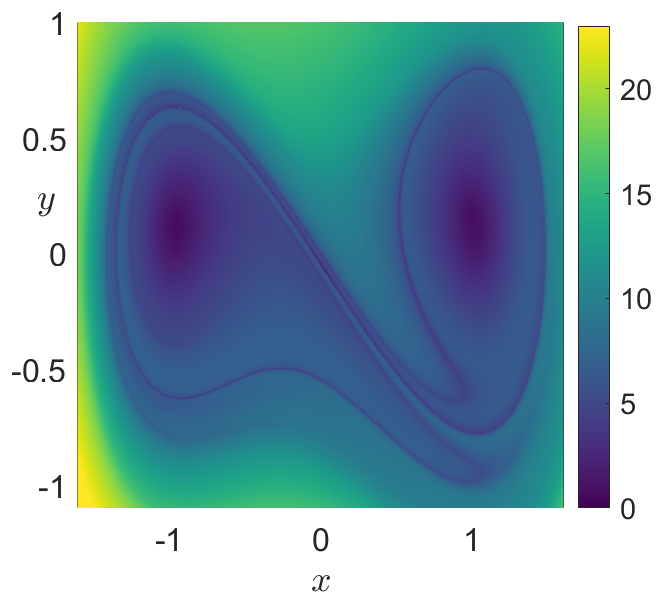
\includegraphics[scale=0.26]{duffing_stbl_tau_10_pert_01.png}
		B)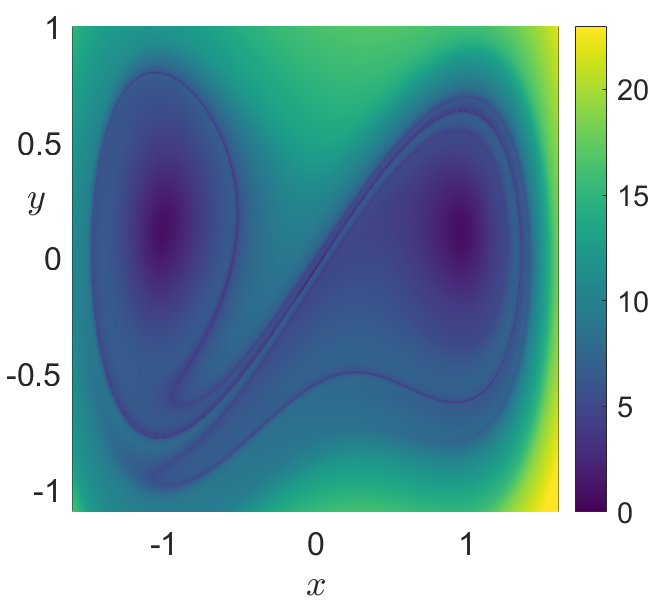
\includegraphics[scale=0.26]{duffing_unstbl_tau_10_pert_01.png}
		C)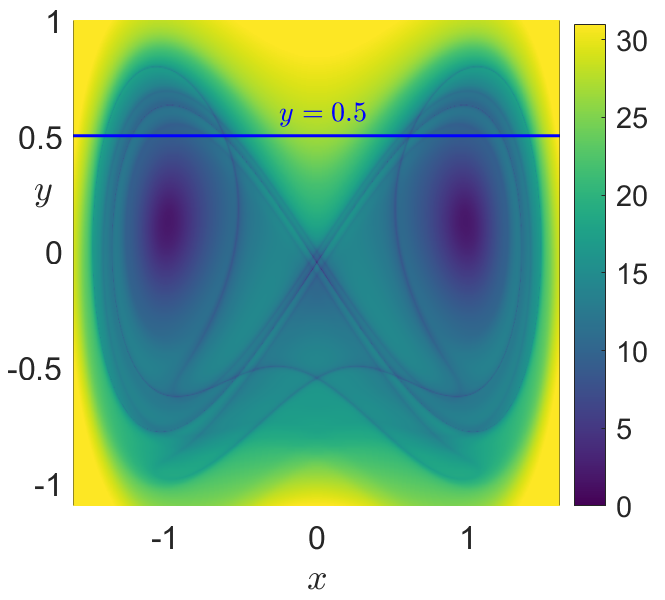
\includegraphics[scale=0.26]{duffing_tau_10_pert_01.png}
		D)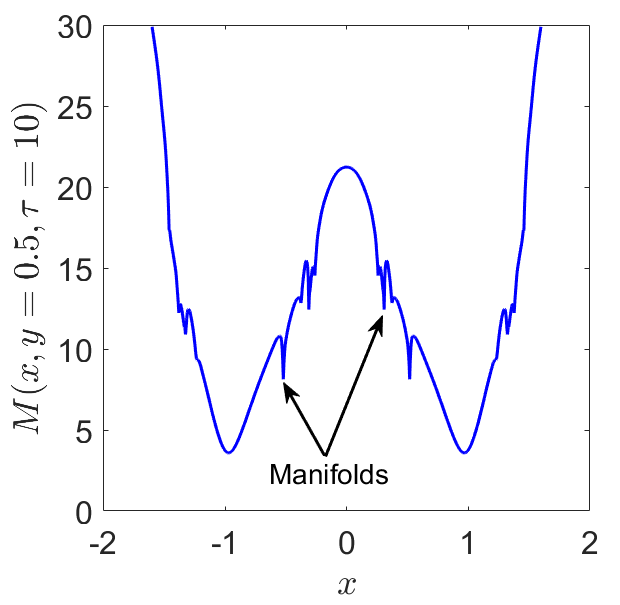
\includegraphics[scale=0.26]{duffing_maniDetect_pert_01.png}
	\end{center}
	\caption{Phase portrait of the nonautonomous and undamped Duffing oscillator obtained at time $t = 0$ by applying the arclength definition of LDs in Eq. \eqref{M_function} with an integration time $\tau = 10$. A) Forward LDs detect stable manifolds; B) Backward LDs highlight unstable manifolds of the system; C) Total LDs (forward $+$ backward) showing that all invariant manifolds are recovered simultaneously. D) Value taken by LDs along the line $y = 0.5$ in panel C) to illustrate how the method detects the stable and unstable manifolds at points where the scalar field changes abruptly.}
	\label{duffing2_lds}
\end{figure}

At this point, we introduce an alternative definition of LDs which was first presented in \cite{lopesino2017} to provide a rigorous theoretical foundation for this methodology, allowing us to establish a mathematical connection between the invariant manifolds in phase space and the ``singular structures'' that appear in the LD scalar field.

\newpage

For high dimensional phase space this approach is problematic and prone to issues of interpretation since a tightly grouped set of initial conditions may result in trajectories that become “lost” with respect to each other in phase space. The method of Lagrangian descriptors turns this problem on its head by emphasizing the initial conditions of trajectories, rather than the precise location of their futures and pasts, after a specified amount of time.  A low dimensional “slice” of phase space can be selected and sampled with a grid of initial conditions of high resolution. Since the phase space structure is encoded in the initial conditions of the trajectories, no resolution is lost as the trajectories evolve in time.

This has been shown to have many advantages over the arclength. For example, it allows for a rigorous analysis of the notion of “singular structures” in certain cases and the relation of this notion to invariant manifolds. It also allows a natural decomposition of the Lagrangian descriptor in a way that isolates distinct dynamical effects. This was utilized in (Demian and Wiggins 2017) in order to show that a Lagrangian descriptor could be used to detect the Lyapunov periodic orbits in the two degree-of-freedom Henon-Heiles Hamiltonian system.








	

One of the biggest challenges when exploring the high-dimensional phase space of a dynamical system is to describe the behavior of ensembles of initial conditions, and to recover from their trajectory evolution the underlying geometrical phase space structures that govern the dynamical mechanisms of the flow. The problem that naturally arises in a   high-dimensional phase space is that the trajectories of ensembles of initial conditions that start nearby might get ``lost'' with respect to each other very quickly, making the use of classical nonlinear dynamics techniques that rely on tracking the location of neighboring trajectories computationally expensive and very difficult to interpret. On the other hand, the method of Lagrangian descriptors provides a revolutionary and radically different approach that resolves this issue, as it focuses on integrating a positive scalar function along the trajectory of any initial condition of the system instead of tracking their phase space location. This is probably one of the key ideas behind the success of this technique, since the phase space geometry is encoded in the initial conditions themselves




In order to explore the phase space structures of the dynamical system given by Hamilton's equations in Eq. \eqref{ham_eqs}, we have used in this work the $p$-norm definition of Lagrangian descriptors introduced in \cite{lopesino2017} with $p = 1/2$. Given an initial condition $\mathbf{x}_0$ at time $t_0$, take a fixed integration time $\tau > 0$ and $p \in (0,1]$. The method is defined as follows:
\begin{equation}
M_p(\mathbf{x}_{0},t_0,\tau) = \int^{t_0+\tau}_{t_0-\tau} \, \sum_{i=1}^{n} |v_{i}(\mathbf{x}(t;\mathbf{x}_0),t)|^p \; dt = M_p^{(b)}(\mathbf{x}_{0},t_0,\tau) + M_p^{(f)}(\mathbf{x}_{0},t_0,\tau) \;,
\label{Mp_function}
\end{equation}
where $M_p^{(b)}$ and $M_p^{(f)}$ represent, respectively, backward and forward integration of the initial condition, that is:
\begin{equation}
M_p^{(b)}(\mathbf{x}_{0},t_0,\tau) = \int^{t_0}_{t_0-\tau} \sum_{i=1}^{n} |v_{i}(\mathbf{x}(t;\mathbf{x}_0),t)|^p \; dt \quad,\quad M_p^{(f)}(\mathbf{x}_{0},t_0,\tau) = \int^{t_0+\tau}_{t_0} \sum_{i=1}^{n} |v_{i}(\mathbf{x}(t;\mathbf{x}_0),t)|^p \; dt
\end{equation}
It is important to highlight that with this definition of LDs one can mathematically prove in Hamiltonian systems that NHIMs and their stable and unstable manifolds are detected as singularities of the $M_p$ scalar field, that is, points at which the function is non-differentiable and thus its gradient takes very large values \cite{lopesino2017,demian2017,naik2019a}. Moreover, in this context it has also been shown that:
\begin{equation}
\mathcal{W}^u(\mathbf{x}_{0},t_0) = \textrm{argmin } M_p^{(b)}(\mathbf{x}_{0},t_0,\tau) \quad,\quad \mathcal{W}^s(\mathbf{x}_{0},t_0) = \textrm{argmin } M_p^{(f)}(\mathbf{x}_{0},t_0,\tau)
\label{min_LD_manifolds}
\end{equation}
where $\mathcal{W}^u$ and $\mathcal{W}^s$ are, respectively, the unstable and stable manifolds calculated at time $t_0$ and $\textrm{argmin}(\cdot)$ denotes the phase space coordinates $\mathbf{x}_0$ that minimize the function $M_p$. In addition, NHIMs at time $t_0$ can be calculated as the intersection of the stable and unstable manifolds:
\begin{equation}
\mathcal{N}(\mathbf{x}_{0},t_0) = \mathcal{W}^u(\mathbf{x}_{0},t_0) \cap \mathcal{W}^s(\mathbf{x}_{0},t_0) = \textrm{argmin} M_p(\mathbf{x}_{0},t_0,\tau)
\label{min_NHIM_LD}
\end{equation}
It is important to point out here that the phase space location of the stable and unstable manifolds can be thus obtained in two ways. First, we can extract them as ridges of the scalar function $||\nabla M_p||$ since manifolds are located at points where the function $M_p$ is non-differentiable. Once the manifolds are known, one can compute the NHIM at their intersection by means of a root search algorithm. The second method to recover the manifolds and their associated NHIM is by minimizing the function $M_p$ using a search optimization algorithm. This second procedure and some interesting variations are described in \cite{feldmaier2019}.


\bigskip
\bigskip

\begin{equation}
M_p(\mathbf{x}_{0},t_0,\tau) = \int^{t_0 + \tau^{+}_{\mathbf{x}_0}}_{t_0 - \tau^{-}_{\mathbf{x}_0}} \sum_{i=1}^{n} |v_{i}(\mathbf{x}(t;\mathbf{x}_0),t)|^p \; dt \;,\quad p \in (0,1] \;.
\label{Mp_vt}
\end{equation}
and, for a fixed integration time $\tau_0 > 0$, the total integration time is defined as:
\begin{equation}
\tau^{\pm}_{\mathbf{x}_{0}} = \min \left\lbrace \tau_0 \, , \, |t^{\pm}|_{\big| \mathbf{x}\left(t^{\pm}; \, \mathbf{x}_{0}\right) \notin \mathcal{R}} \right\rbrace \; ,
\end{equation}
where $t^{+}$ and $t^{-}$ are the times for which the trajectory leaves the interaction region $\mathcal{R}$ in forward and backward time, respectively. For the analysis of the Caldera-type Hamiltonian in this work we have chosen:
\begin{equation}
\mathcal{R} = \left\lbrace \mathbf{x} = (x,y,p_x,p_y) \in \mathbb{R}^4 \; \big| \; |y| \leq 6 \right\rbrace \;.
\label{inter_reg}
\end{equation}
We conclude the description of the method by highlighting the fact  that if the selected interaction region is large enough, the variable integration time LD definition given above in Eq. \eqref{Mp_vt} will approach the fixed-time LD definition in Eq. \eqref{Mp_function}. Thus, NHIMs and their stable and unstable manifolds will be captured by the phase space points for which the LD is non-differentiable and local minimum behavior given in Eqs. \eqref{min_LD_manifolds} and \eqref{min_NHIM_LD} is recovered. Consequently, the variable integration time LD provides us with a suitable methodology to study the phase space geometrical structures that characterize the dynamics in open potentials, since it avoids the issue of trajectories escaping to infinity very fast.

To finish this section we will illustrate how variable integration time LDs can be used to detect the geometrical phase space structures, that is, the NHIMs and their stable and unstable invariant manifolds that characterize the dynamical matching phenomenon in the Caldera Hamiltonian system. In particular, we will focus on the extraction of the phase space structures for the dynamical system given in Eq. 

Once we have fixed the phase space slice where we want to compute LDs, we select a grid of initial conditions and, after discarding those that are energetically unfeasible, we integrate the remaining conditions both forward and backward in time, and compute LDs using the definition in Eq. \eqref{Mp_vt} with $p = 1/2$ along the trajectory for the whole fixed integration time or until the initial condition leaves the interaction region $\mathcal{R}$ in Eq. \eqref{inter_reg}, what happens first. The result is that if we plot the LDs values obtained from the forward/backward integration, the scalar field will reveal the stable/unstable manifolds in the SOS under consideration. Moreover, if we plot the combined sum of forward and backward integration, the method highlights both stable and unstable manifolds simultaneously. We can clearly see that the manifolds are detected at points where the LD scalar function is non-differentiable. Therefore, we can directly extract the invariant stable and unstable manifolds in the SOS from the gradient, that is, using $||\nabla \mathcal{M}_p||$. It is important to note here the crucial role that the integration time $\tau$ plays when it comes to revealing the invariant manifolds in phase space. when we increase the value for the integration time, richer and more complex details of the underlying geometrical template of phase space structures is unveiled. This behavior is expected, since an increase of the integration time would imply incorporating more information about the past and future dynamical history of particle trajectories in the computation of LDs. This means that $\tau$ is intimately related to the time scales of the dynamical phenomena that take place in the model under consideration and thus, it is a parameter that is problem-dependent. Consequently, there is no general ``golden'' rule for selecting its value for exploring phase space, and thus it is usually selected from the information obtained by performing several numerical experiments. One needs to always bare in mind that there is a compromise between the complexity of the structures that one would like to reveal to explain a certain dynamical mechanism, and the interpretation of the intricate manifolds displayed in the LD scalar output. 

As a final remark to complete the analysis of this example on how the method of Lagrangian descriptors is applied to extract the geometrical template of invariant manifolds in a high-dimensional phase space by means of looking at low-dimensional slices, there is a key point that needs to be highlighted and that demonstrates the real potential of LDs with respect to other classical techniques from nonlinear dynamics. Using LDs we can obtain \textit{all} the manifolds coming from \textit{any} NHIM in phase space \textit{at the same time}. This is of course a tremendous advantage in comparison to the classical approach of computing stable and unstable manifolds that relies on locating first the NHIMs in phase space individually, and for every NHIM globalize the manifolds separately, for which a knowledge of the eigendirections is crucial. Consequently, the application of LDs offers the capability of recovering \textit{all} the relevant phase space structures in one \textit{shot} without having to study the local dynamics about equilibrium points of the dynamical system.

\bigskip
\bigskip

\begin{equation}
H = \dfrac{p_x^2}{2m_x} + \dfrac{p_y^2}{2m_y} + \dfrac{\lambda^2}{2} x^2 - \dfrac{\omega^2}{2} y^2 \quad \Leftrightarrow \quad
\begin{cases}
\dot{x} = \dfrac{p_x}{m_x} \\[.3cm]
\dot{p}_{x} = \lambda^2 x \\[.3cm]
\dot{y} = \dfrac{p_y}{m_y} \\[.3cm]
\dot{p}_{y} = -\omega^2 y 
\end{cases}
\label{index1_Ham}
\end{equation}

\bigskip
\bigskip
\bigskip
\bigskip

\begin{figure}[htbp]
	\begin{center}
		A)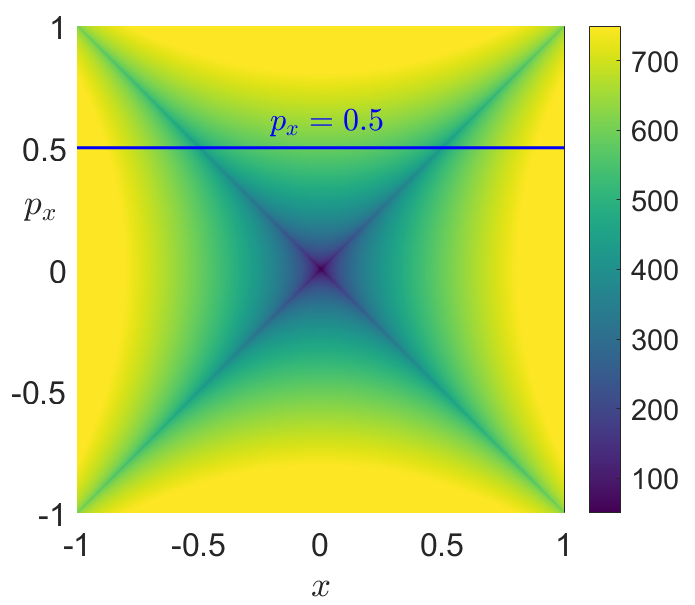
\includegraphics[scale=0.24]{LD_p_05_Saddle_tau_10.png}
		B)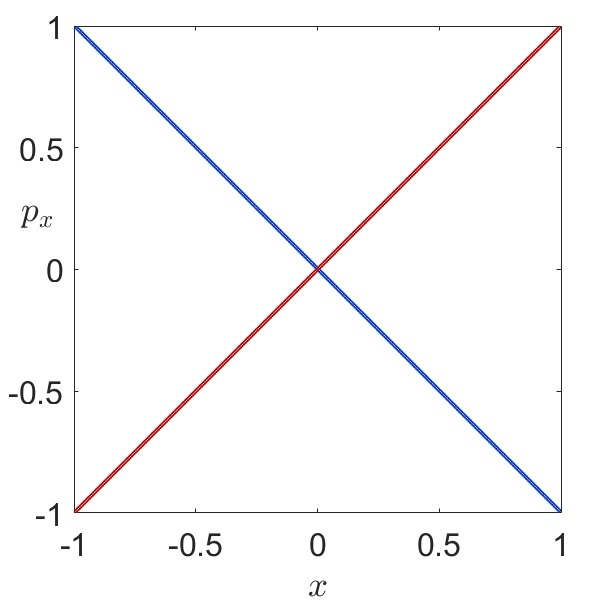
\includegraphics[scale=0.24]{manifolds_Saddle_tau_10.png}
		C)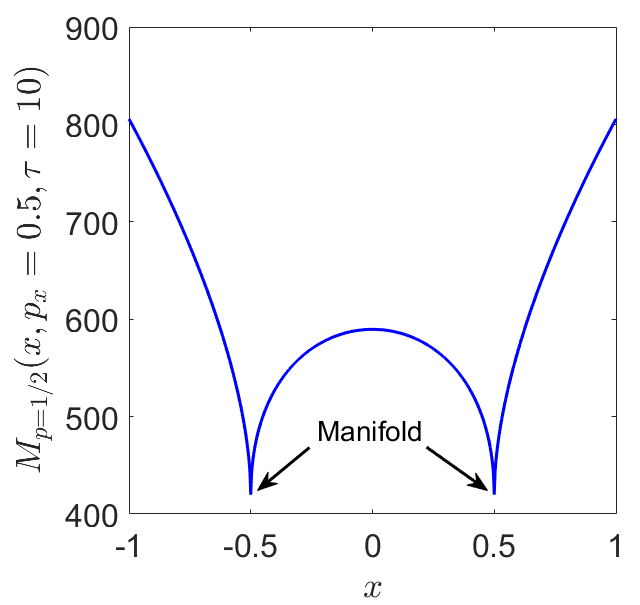
\includegraphics[scale=0.24]{detectMani_Saddle_tau_10.png}
	\end{center}
	\caption{Phase portrait in the saddle space of the linear Hamiltonian given by Eq. \eqref{index1_Ham}, associated to an index-1 saddle. A) Applicaton of the $p$-norm definition of LDs in Eq. \eqref{Mp_function} using $p = 1/2$ with $\tau = 10$; B) Invariant stable (blue) and unstable (red) manifolds of the unstable periodic orbit at the origin extracted from the gradient of the $M_p$ function; C) Value of LDs along the line $p_x = 0.5$ depicted in panel A) to illustrate how the method detects the stable and unstable manifolds at points where the scalar field is singular or non-differentiable.}
	\label{index1_lds}
\end{figure}


\bigskip
\bigskip
\bigskip
\bigskip

\begin{equation}
H = \dfrac{1}{2} p_x^2 + \dfrac{1}{2} x^2 + \dfrac{1}{3} x^3 \quad \Leftrightarrow \quad
\begin{cases}
\dot{x} = p_x \\
\dot{p}_{x} = - x - x^2
\end{cases}
\label{fish_Ham}
\end{equation}

We have used the interaction region as a circle of radius 15 centered at the origin.

\bigskip
\bigskip
\bigskip
\bigskip

\begin{figure}[htbp]
	\begin{center}
		A)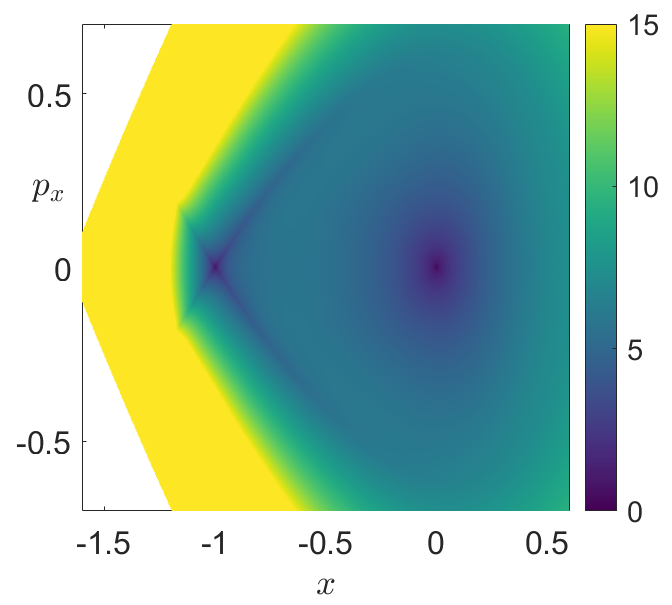
\includegraphics[scale=0.24]{LDfixTime_p_05_fishPot_tau_3.png}
		B)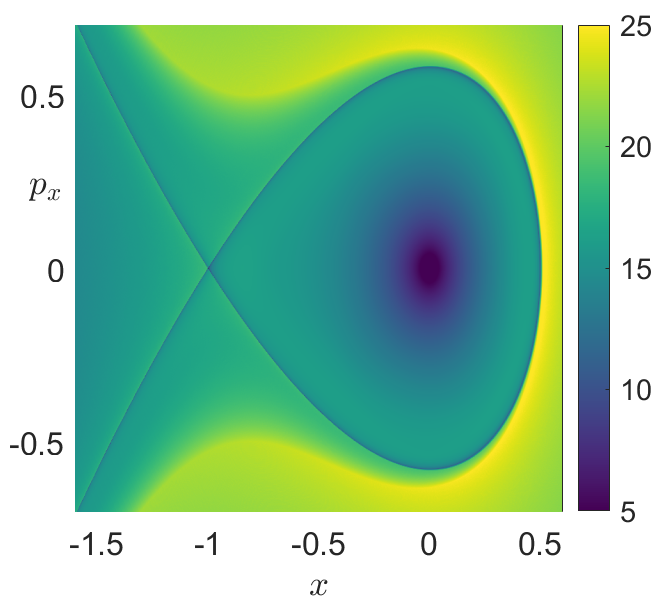
\includegraphics[scale=0.24]{LD_p_05_fishPot_tau_8.png}
		C)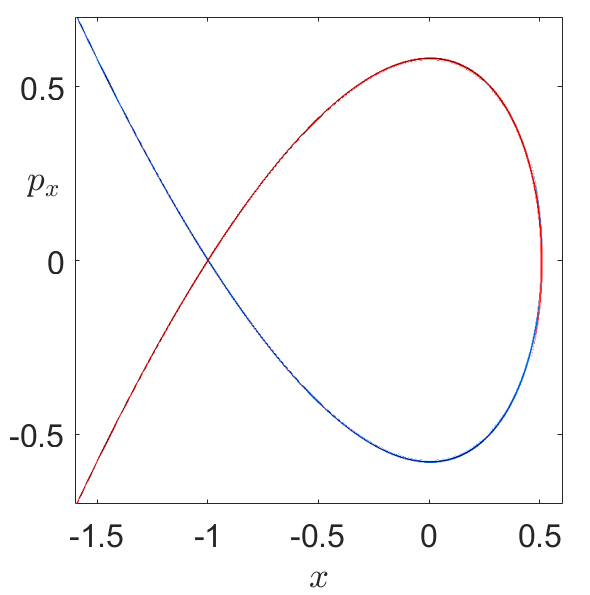
\includegraphics[scale=0.24]{manifolds_fishPot_tau_8.png}
	\end{center}
	\caption{Phase portrait of the ``fish potential'' Hamiltonian given by Eq. \eqref{fish_Ham} revealed by the $p$-norm LDs with $p = 1/2$. A) Applicaton of the fixed time integration definition of LDs in Eq. \eqref{Mp_function} with $\tau = 3$; B) Variable time integration definition of LDs in Eq. \eqref{Mp_vt} with $\tau = 8$; C) Invariant stable (blue) and unstable (red) manifolds of the saddle fixed point  extracted from the gradient of the variable time $M_p$ function.}
	\label{fish_lds}
\end{figure}


In order to illustrate how LDs reveal geometry of invariant manifolds in a high-dimensional phase space we will apply it to the classical H\'enon-Heiles


\begin{figure}[htbp]
	\begin{center}
		A)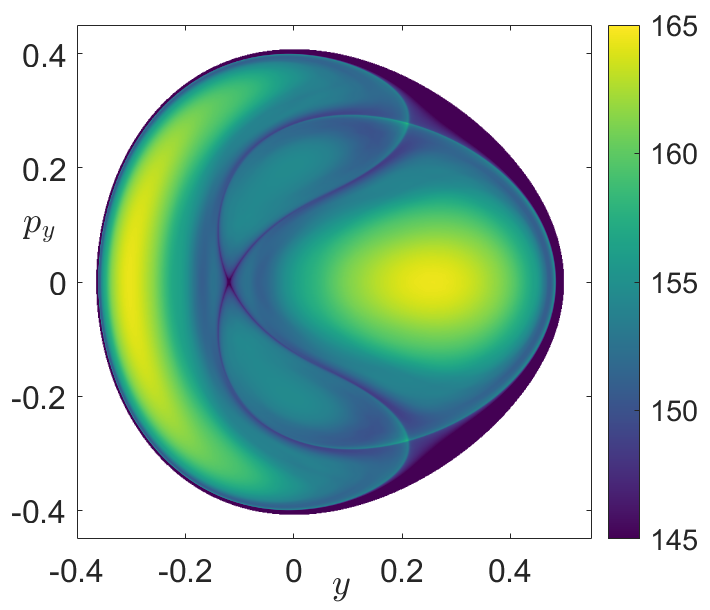
\includegraphics[scale=0.35]{LDs_Henon_tau_50_x_0_E_1div6.png}
		B)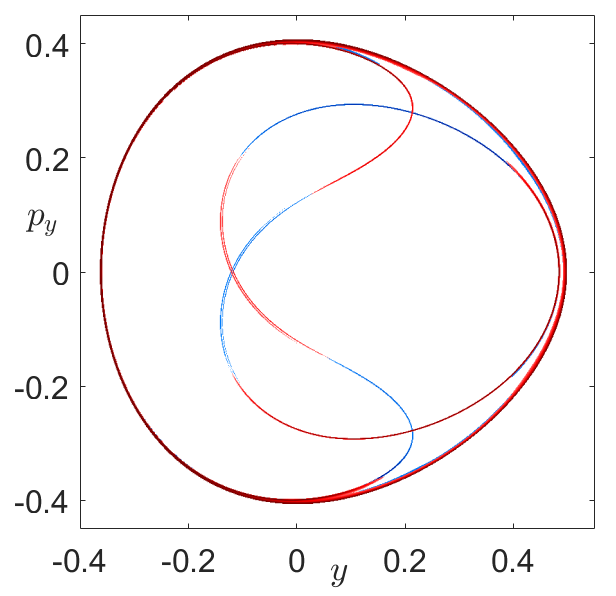
\includegraphics[scale=0.35]{Mani_Henon_tau_50_x_0_E_1div6.png}
		C)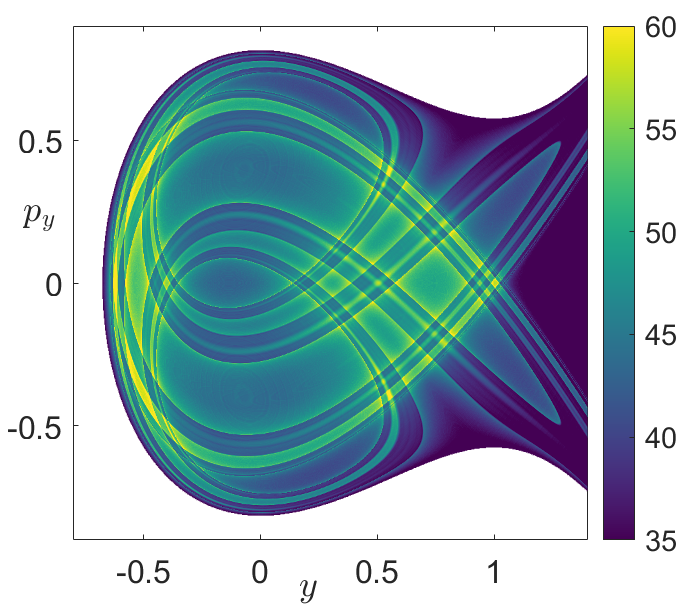
\includegraphics[scale=0.36]{LDs_Henon_tau_10_x_0_E_1div3.png}
		D)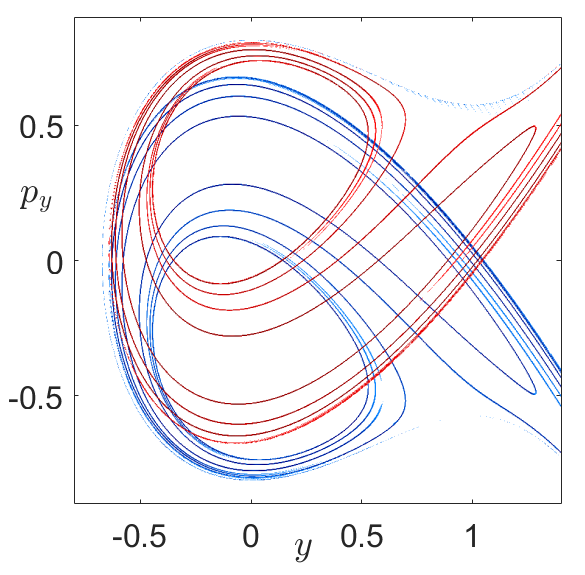
\includegraphics[scale=0.36]{Mani_Henon_tau_10_x_0_E_1div3.png}
		E)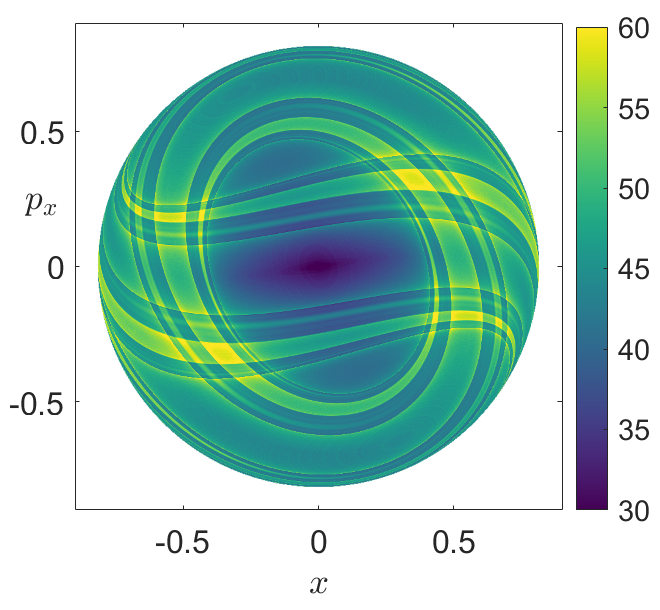
\includegraphics[scale=0.36]{LDs_Henon_tau_10_y_0_E_1div3.png}
		F)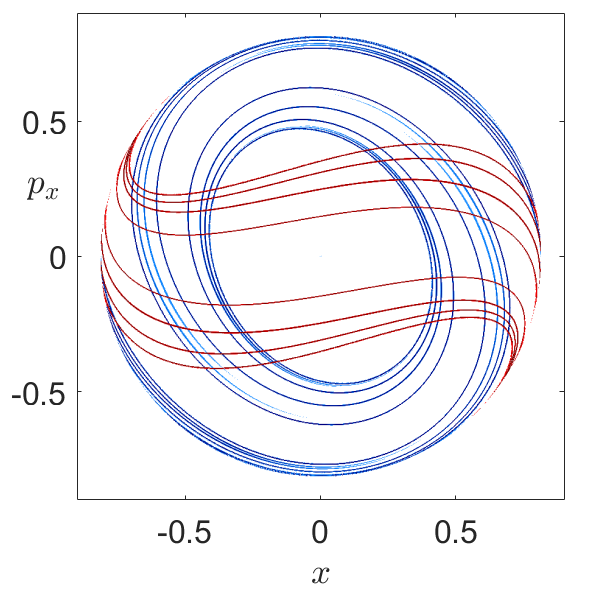
\includegraphics[scale=0.36]{Mani_Henon_tau_10_y_0_E_1div3.png}
	\end{center}
	\caption{Phase space structures of the H\'enon-Heiles Hamiltonian revealed by the variable time $p$-norm LDs with $p = 1/2$. A) Invariant stable (blue) and unstable (red) manifolds extracted from the gradient of the variable time $M_p$ function.}
	\label{henonHeiles_lds}
\end{figure}

As we have mentioned before, NHIMs and their associated stable and unstable manifolds play a crucial role for the analysis of transition dynamics across index-1 saddles that separate two neighboring wells of a PES. This situation is representative for example in chemical isomerization problems, where two wells corresponding to different stable configurations of a given molecule are separated by an energy barrier that the system has to cross in order to undergo an isomerization reaction. In this context, several numerical studies have been carried out recently by means of Lagrangian descriptors to analyze escaping dynamics on open PESs \cite{demian2017,naik2019b,GG2019}. 

At this point, it becomes clear from our discussion that the development of nonlinear techniques that have the capability of unveiling the high-dimensional phase space structures that characterize reaction mechanisms is of paramount importance. The methodology offered by LDs in this respect has been shown to have many advantages. For instance, it is straightforward to implement and computationally inexpensive when applied to systems with two or three DoF. But probably the most important feature of this tool is that it allows to produce a complete and detailed geometrical \textit{phase space tomography} in high dimensions by means of using low-dimensional phase space probes to extract the intersections of the phase space invariant manifolds with these slices \cite{demian2017,naik2019a,naik2019b,GG2019}. 

To finish this section we will illustrate how LDs can be used to detect the geometrical phase space structures, that is, the NHIMs and their stable and unstable invariant manifolds that characterize reaction dynamics between different wells of a PES separated by index-1 saddles.


We start our explanation on how to use the method of Lagrangian descriptors by computing it on the Poincar\'e SOS in Eq. \eqref{psos_ld} for the uncoupled system, i.e. $\beta = 0$, using a small integration time $\tau = 5$. Once we have fixed the phase space slice where we want to calculate LDs, we select a grid of initial conditions and, after discarding those that are energetically unfeasible, we integrate the remaining conditions both forward and backward in time, and compute LDs using the definition in Eq. \eqref{Mp_function} with $p = 1/2$. The result is that if we plot the LDs values obtained from the forward/backward integration, the scalar field will reveal the stable/unstable manifolds in the SOS under consideration. Moreover, if we plot the combined sum of forward and backward integration, the method highlights both stable and unstable manifolds simultaneously. We can clearly see that the manifolds are detected at points where the LD scalar function is non-differentiable. the values taken by the LD function along the line $p_x = 0.2$. Notice the jumps in the values of the function, which indicate non-differentiability by means of very large gradient values. Therefore, we can directly extract the invariant stable and unstable manifolds in the Poincar\'e SOS from the gradient, that is, using $||\nabla \mathcal{M}_p||$. 

 One needs to always bare in mind that there is a compromise between the complexity of the structures that one would like to reveal to explain a certain dynamical mechanism, and the interpretation of the intricate manifolds displayed in the LD scalar output. 




As a final remark, there is a key point that needs to be highlighted with regard to the application of LDs and that demonstrates the real potential of this tool with respect to other classical nonlinear dynamics techniques. We have seen that one can extract the stable and unstable manifolds from the gradient of the $M_p$ function and therefore obtain \textit{all} the manifolds coming from \textit{any} NHIM in phase space \textit{at the same time}. This is of course a tremendous advantage in comparison to the classical approach of computing stable and unstable manifolds that relies on locating first the NHIMs in phase space individually, and for every NHIM globalize the manifolds separately, for which a knowledge of the eigendirections is crucial. Consequently, the application of LDs offers the capability of recovering \textit{all} the relevant phase space structures in one \textit{shot} without having to study the local dynamics about equilibrium points of the dynamical system.

\smallskip

To finish this chapter we would like to mention that the method of Lagrangian descriptors has also been adapted to explore the template of geometrical structures present in the phase space of stochastic dynamical systems \cite{balibrea2016lagrangian}. This achievenment clearly evidences the versatility that this mathematical technique brings to the nonlinear dynamics community. We are confident that the analysis of stochastic processes that play a crucial role in chemical reaction dynamics by means of LDs will surely help to shed light and provide new and interesting insights in the development of Chemistry. Definitely, Lagrangian descriptors is the ultimate tool to reveal the strong bond that exists between Chemistry and Mathematics in phase space.





\bibliography{LDs}

\end{document}

